\clearpage
\chapter{Introduction}

Clinicians monitor gliomas with repeated magnetic resonance imaging (MRI), comparing scans to assess disease status and treatment response. Earlier scans give a record of the changes leading up to the current visit. We wanted to know whether a model could use that history to predict later anatomy more accurately than a model given only the latest scan.

\section{Learning a patient state}

A world model represents a system's state and predicts how that state changes, potentially conditioned on actions \cite{ref2}. For longitudinal MRI, that meant learning a patient state from the scans available at a visit and, in some experiments, recorded clinical information. We checked what the state retained by decoding compartment volumes and segmentation masks and comparing them with the references from the same visit.

We started with a Joint-Embedding Predictive Architecture (JEPA) \cite{ref3}. Its MRI encoder produced a feature vector for each visit, and a temporal predictor used the observed visits to predict the features of a later one. To check what these predictions meant anatomically, we fitted readouts that converted them into compartment volumes. In the initial evaluation, copying the measured current volumes gave lower error than the JEPA forecast. That result alone did not tell us whether the representation was losing anatomy, the predictor was failing to model change, or both.

The later spatial encoders kept a grid of features and were trained to predict masks and volumes from the current MRI. We also tried giving forecasting models the volumes measured from the masks directly, along with their previous changes. These forecasts could test whether history helped without relying on an MRI encoder to estimate the input volumes.

\section{Testing the contribution of history}

Persistence copies the current volume or segmentation to the future visit. A model could beat persistence using only the current scan, so this comparison alone would not tell us whether earlier scans helped. We therefore also used a matched latest-only model that received the current MRI-derived state and the same other inputs, but none of the earlier MRI features. When models received measured volumes, the current-only control left out previous measured change.

We reported measured-volume and decoded-state persistence separately: the first uses volumes from current masks, while the second uses estimates recovered from MRI and therefore includes estimation error. For distributional forecasts, we also used probabilistic scores to assess accuracy and uncertainty.

\section{Data and scope}

LUMIERE \cite{ref4} was the main development dataset. We used SAILOR \cite{ref18} to examine transfer to another longitudinal MRI cohort. Both supplied anatomical references from automated segmentations. Later experiments used MU-Glioma-Post \cite{ref19}, which supplied neuroradiologist-reviewed masks and a separate resection-cavity label. The main compartments were enhancing tumor, necrotic or nonenhancing tissue, and edema or fluid-attenuated inversion recovery (FLAIR) abnormality, with definitions specific to each dataset.

Follow-up was irregular. Predicting the next observed visit without knowing its date is a different task from predicting anatomy at a supplied interval. Chapter~\ref{ch:design} states which experiments were given the future interval retrospectively. Future MRI and masks were excluded from predictor inputs. Treatment records were incomplete, and acquisition differences could also affect the apparent change between scans.

Fitting and scoring used different patients within each comparison. Results from these cohorts still informed later experiments, including the SAILOR transfer studies, so the findings remain development evidence. The forty reserved MU-Glioma-Post patients remain unopened.

Some models improved current-anatomy estimates, but the tested comparisons did not establish a consistent, practically useful forecasting gain from earlier MRI history.

Figure~\ref{fig:1.1} shows one LUMIERE patient's FLAIR scans and automated compartment contours at three visits. The volumes below each scan come from the full masks, including tissue outside the displayed slice.

\begin{figure}[htbp]\centering
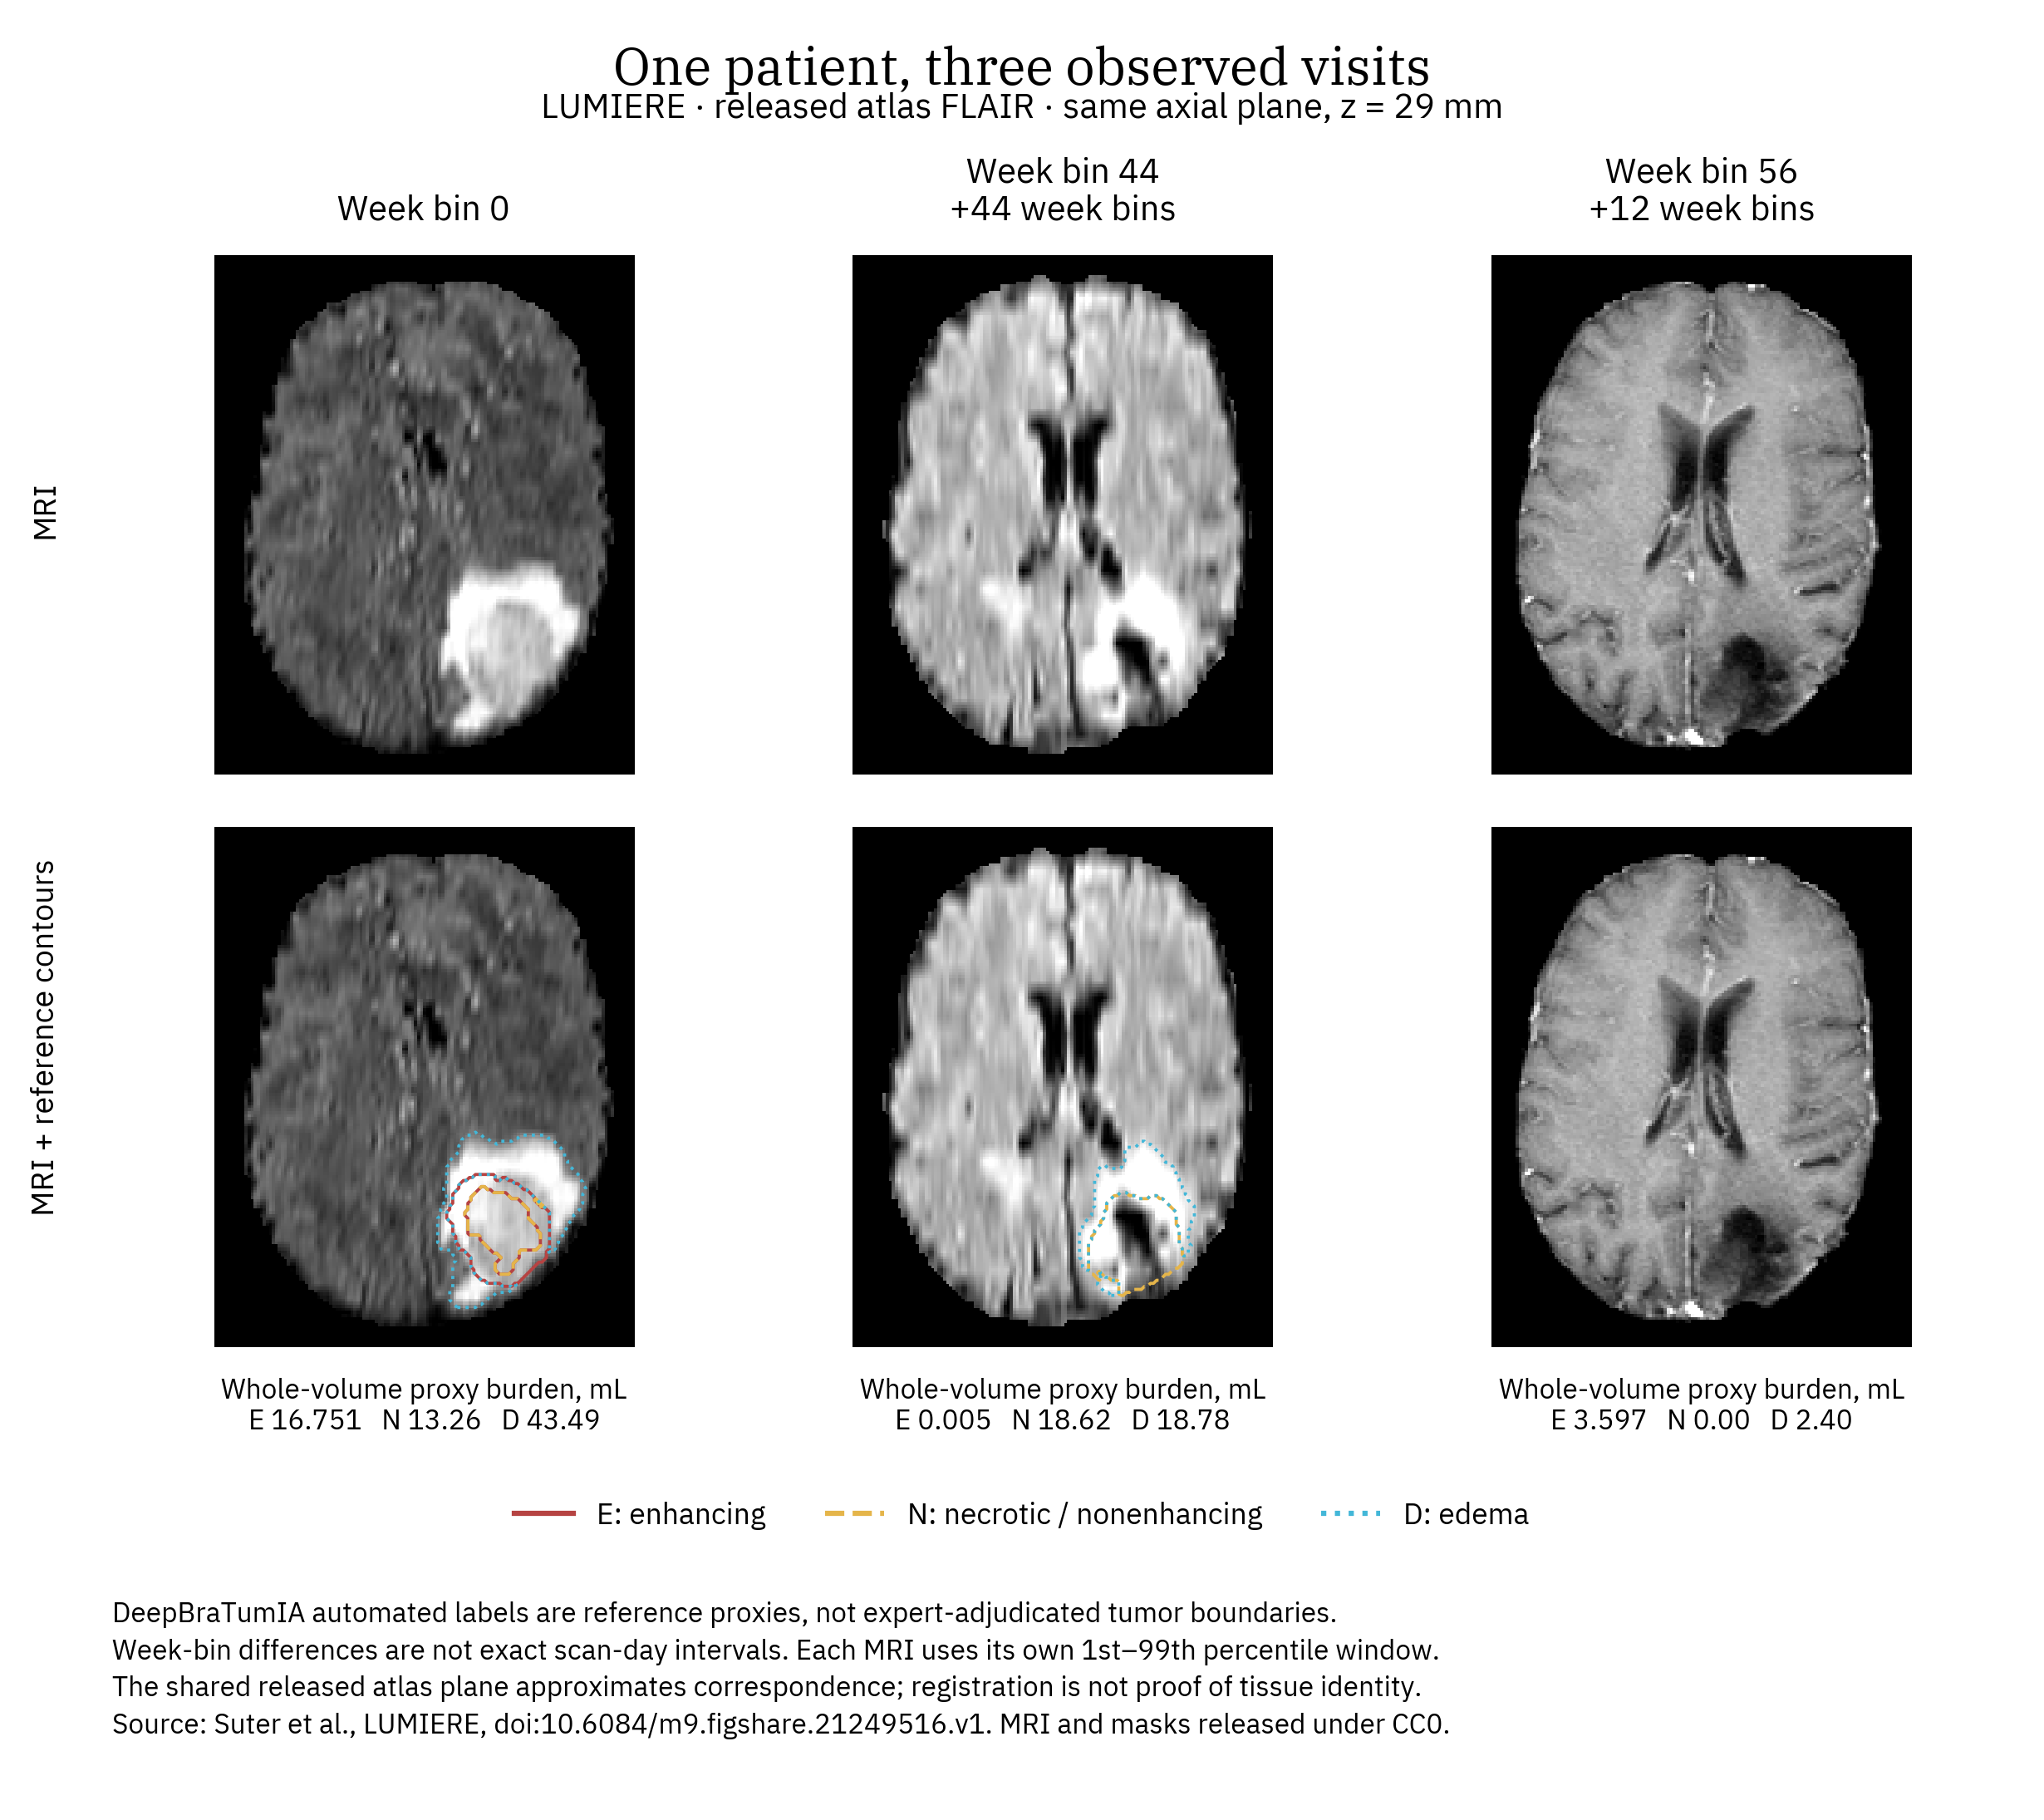
\includegraphics[width=\linewidth,height=0.55\textheight,keepaspectratio]{figures/figure_1_1.png}
\caption[Longitudinal FLAIR MRI and automated reference compartments]{FLAIR MRI and automated DeepBraTumIA compartments at week bins 0, 44 and 56, on the released atlas plane $z = 29$ mm. We selected the first patient in sorted order and the first complete visit in each of that patient's first three distinct week bins. The common slice maximizes summed reference foreground area across these visits. Week bins do not specify exact scan-day intervals, and the displayed visits need not be consecutive clinical examinations. Source: Suter et al., LUMIERE MRI and automated segmentations \cite{ref17}; CC0 1.0.}\label{fig:1.1}
\end{figure}
